\graphicspath{{figure/chap3/}}
\chapter{光的衍射}

\section{夫琅禾费单缝衍射}

\subsection{衍射现象概述}
当光波遇到障碍物,将或多或少地偏离几何光学的直线传播而绕行,这种现象统称为光的衍射.衍射使光强可以波及几何阴影区内,衍射也可以使几何照明区内出现暗纹或暗斑.总之,衍射效应使屏障以后的空间光强分布,既区别于几何光学给出的光强分布,又区别于光波自由传播时的光强分布,衍射光强有了一种重新分布.

衍射是一切波动均具有的传播行为.然而光波衍射却不易为人们所觉察,这有两点原因,一是可见光的波长极短,二是普通光源是非相干的面光源,当我们用一束高亮度的光束,照射各种形状且线度较小的开孔或屏障时,在较远的屏幕上,将呈现不同的衍射图样。

\insertfig{3-1.png}{各种衍射图样}{1}

衍射现象具有两个鲜明特点。其一是，当光束在衍射屏上的某一方位受到限制时，远处屏幕的衍射光强就沿着这个方向扩展开来，也就是说波具有顽强的反限制的特征。二是光孔限度与光波长之比是一个敏感因素，这一点可以用一个统一的公式来反映:
\[
\rho \Delta \theta \approx \lambda
\]

其中$\lambda$为光的波长，$\Delta \theta$为中心衍射斑的角宽度，$\rho$为狭缝的宽度。其中$\Delta \theta$越大，说明衍射效应越强，因此我们可以简单地说，狭缝宽度越小，衍射现象越明显，中心衍射斑铺展的越开。上面这个式子我们会在后面给出推导。

\insertfig{3-2.png}{用激光束观察衍射现象}{0.5}

\subsection{惠更斯-菲涅耳原理}

在正式阐述这一理论之前，我们先提请读者回忆在力学中曾经学习过的球面简谐波的波函数和复数表示法，它们对我们接下来的论述是有意义的。对于这部分不清楚的读者可以参阅大学物理力学部分的教科书，这里不再赘述。

对于点源在原点的球面波，其波函数可以被写为:
\[
U(r,t) = \frac{A}{r}\cos(\omega t-kr-\varphi_0)
\]
复数形式为:
\[
U(r,t) = \frac{A}{r}e^{ikr}\cdot e^{-i\omega t}
\]

\insertfig{3-3.png}{衍射积分式中各量的说明}{0.4}

下面阐述这原理的具体内容.用简短的文字概括起来,惠更斯-菲涅耳原理可表述如下:波前$\Sigma$上每个面元$\d \Sigma$都可以看成是新的振动中心,它们发出次波。在空间某一点$P$的振动是所有这些次波在该点的相干叠加。写成公式是:
\[
U(P) = \oiint_{\Sigma} \d U =  K \oiint_{\Sigma} f(\theta_0,\theta)U_0(Q)\frac{e^{ikr}}{r}\d S
\]
这公式中的各个符号可以被解释如下:$\d S$代表着微分面元; $U_0(Q)$是这些次波源本身的复振幅; $\frac{e^{ikr}}{r}$代表次波源发射球面波到达场点;$f(\theta_0,\theta)$被称为倾斜因子，用于表示次波源的发射并非各项同性。

基尔霍夫在大约这个公式提出的六十年后从定态波场的亥姆霍兹方程出发，利用矢量场论中的格林公式在$r\gg \lambda$条件下导出了无源空间边值定解的表达式:
\[
U(P) = \frac{-i}{\lambda} \oiint_{\Sigma} \frac{(\cos\theta_0+\cos\theta)}{2}U_0(Q)\frac{e^{ikr}}{r}\d S
\]

写成实数形式是:
\[
E(P,t) = \int_S \frac{E(Q)K(\varphi)}{r} \cos(\omega t-kr)\d S
\]

其中$P$为场点，$Q$为波前上一点，$K(\varphi)$为倾斜因子。

\insertfig{3-4.png}{衍射系统的分类}{0.8}

衍射系统以衍射屏幕为界，可以被分为前场和后场。在无成像的衍射系统中，通常按照光源，衍射屏，接收屏三者之间距离的远近分为菲涅耳衍射(图(a))和夫琅禾费衍射(图(b))。菲涅耳衍射是指，光源-衍射屏或者衍射屏-接收屏两者距离中至少有一个为有限远的衍射系统。夫琅禾费衍射则指的是衍射屏与光源和接收屏均是无限远的情形。简单而言，菲涅耳衍射是近场衍射，夫琅禾费衍射是远场衍射。

当然上面的分类也不尽准确，对于夫琅禾费衍射，我们常常使用透镜接收后场中的衍射光波并使其在透镜的后焦面上形成衍射光斑。

对于菲涅耳衍射，最著名的莫过于菲涅耳圆盘衍射产生的光斑。经过理论计算后菲涅耳指出，在使用一个遮光圆盘作为衍射屏时，接收面的中心会出现一个亮斑。这结论看起来不可思议，但是得到了实验证实。事实上，现在我们更多使用的还是夫琅禾费衍射，我们在下节内容中予以详细介绍。

\subsection{夫琅禾费单缝衍射}

\insertfig{3-5.png}{夫琅禾费衍射装置}{0.6}
夫琅禾费单缝衍射的装置如图所示.用平行光照射单缝，在透镜后焦面上接收衍射光波，单缝的宽度$a$远小于垂直纸面的长度$b$,这样衍射强度将显著地沿着$x$方向扩展。

为了求解衍射强度的分布，我们采用如下的方法:将缝面处的波阵面划分为$N$个与狭缝平行的等宽窄条,其中$N$非常大。注意到窄条发出的子波在$P$点的光振动产生的振幅近似相等，设为$E_0$。狭缝最边缘的两个窄条$A,B$发出的衍射光到达$P$点时的光程差$AC= a\sin\theta$。相邻的两个窄条发出的子波在$P$点的光程差为$\frac{a\sin\theta}{N}$，相位差为$\Delta \varphi =\frac{2\pi}{\lambda}\cdot \frac{a\sin\theta}{N}$.

因此点$P$处的光振动可以被视为$N$个同频率同振幅振动方向相同，相位依次相差一个恒量$\Delta \varphi=\frac{2\pi}{\lambda}\cdot\frac{a\sin\theta}{N}$.如图所示$N\to\infty$时，$N$个相接的折线将变为一个圆弧。

\begin{figure}[htbp]
    \centering
    % 第一张图
    \begin{minipage}[b]{0.48\textwidth}
        \centering
        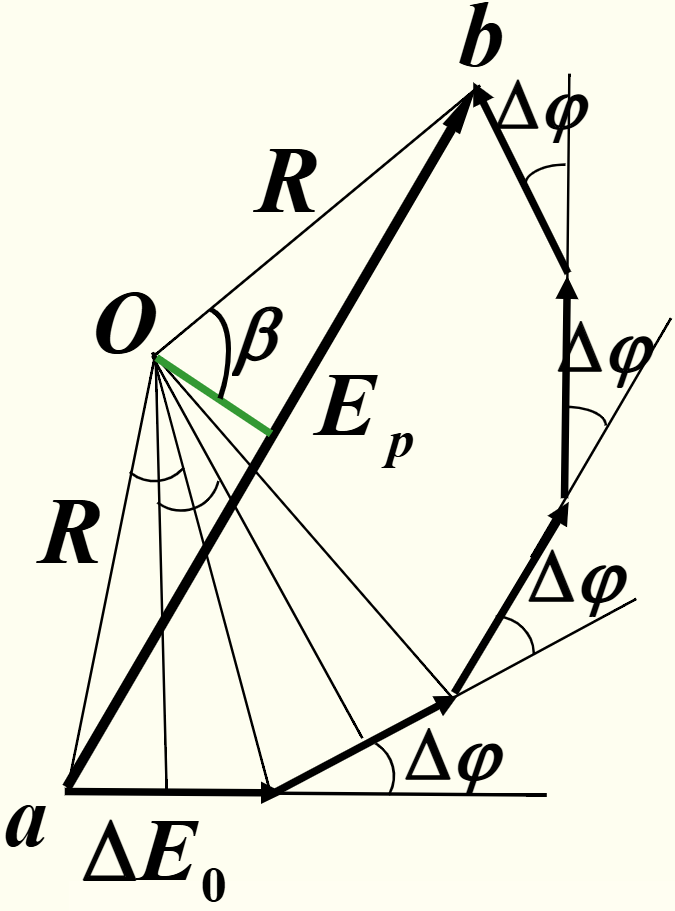
\includegraphics[width=0.55\textwidth]{3-6.png} % figure/image1.png
        \caption{振幅矢量法合成振幅}
    \end{minipage}
    \hfill
    % 第二张图
    \begin{minipage}[b]{0.48\textwidth}
        \centering
        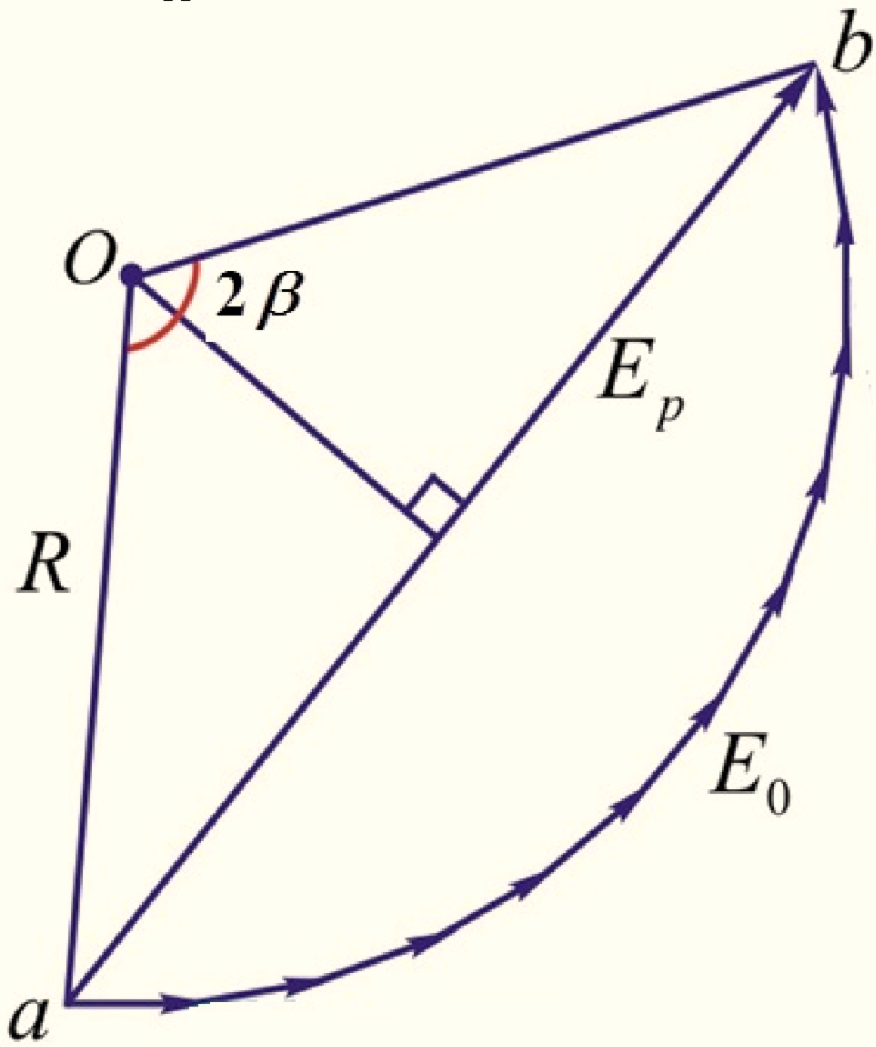
\includegraphics[width=0.55\textwidth]{3-7.png} % figure/image2.png
        \caption{$N \to \infty$时变为圆弧}
    \end{minipage}
\end{figure}

由几何关系:
\[
\beta = N\cdot \Delta \varphi= \frac{\pi a \sin\theta}{\lambda}, \quad E_p =2R\sin\beta, E_0 = 2R\beta\Rightarrow \frac{E_p}{E_0}=\frac{\sin \beta}{\beta}
\]

注意到光强与振幅的平方成正比，因此我们可以得到$P$点的光强:
\[
I = I_0(\frac{\sin\beta}{\beta})^2
\]

其中$I_0$为入射光强。

在这之后我们将多次遇见$\frac{\sin x}{x}$型函数，可以记作$\mathrm{sinc}(x)$.我们对这函数的一些性质在下面做些阐述。

\insertfig{3-8.png}{$\mathrm{sinc}(x)$图象}{0.65}

\insertfig{3-9.png}{$\mathrm{sinc}^2(x)$图象}{0.7}

(1)最大值(主极大). 当$x=0$,$\mathrm{sinc}(x)=\frac{\sin x}{x}=1$时为最大值.这在单缝衍射中，表现为$\theta=0$时，衍射强度$I(0)=I_0$为最大值，称其为零级衍射峰，其位置正是几何光学像点位置。这个位置也被称为单缝中央主极大光强，也被称为中央明纹中心。

(2)零点位置. $\mathrm{sinc}(x)$函数存在一系列零点.当$x=k\pi,k=\pm 1, \pm 2,\dots$时，$\mathrm{sinc}(x)=0$.这在单缝衍射中，表现为当:
\[
a\sin\theta = k\lambda , \quad k = \pm 1, \pm 2,\dots
\]
时，衍射强度$I(\theta)=0$,出现暗纹。上式称为单缝衍射零点条件。

(3)次极大. $\mathrm{sinc}$函数在相邻两个零点间存在一个极大值，这个位置由:$\frac{\d(\mathrm{sinc}(x))}{\d x} = 0 \Rightarrow x = \tan x$这个超越方程给出，其数值结果可以被列表如下:

\begin{table}[h!]
\centering
\renewcommand{\arraystretch}{1.8} % 行距
\setlength{\tabcolsep}{18pt}      % 列间距

\begin{tabular}{|c|c|c|c|}
\hline
$x$ 
& $\pm 1.43\pi$ 
& $\pm 2.46\pi$
& $\pm 3.47\pi$ \\
\hline
$\sin\theta$ 
& $\pm 1.43\,\frac{\lambda}{a}$ 
& $\pm 2.46\,\frac{\lambda}{a}$ 
& $\pm 3.47\,\frac{\lambda}{a}$ \\
\hline
\multirow{2}{*}{$\operatorname{\mathrm{sinc}}(x)$}
& 0.22 & 0.13 & 0.09 \\
\cline{2-4}
& $4.7\%$ & $1.7\%$ & $0.8\%$ \\
\hline
\end{tabular}

\end{table}

我们可以发现在次极大上的光强非常少，零级衍射斑集中了全部入射功率的$80\%$以上，因此我们常常用下面的半角宽度来表征衍射的强度。

(4)半角宽度. 零级衍射斑的角范围由零级衍射峰与其相邻暗点之间的角方位的差值予以度量，称其为零级衍射的半角宽度。$\Delta \theta_0 = \theta_1-\theta_0$. 在平行光正入射条件下，$\theta_0=0$,$\theta_1\approx \sin \theta_1 =\frac{\lambda}{a}$. 因此半角宽度为:
\[
\Delta \theta_0 = \frac{\lambda}{a} , \quad a \cdot \Delta \theta_0 = \lambda
\]

在进行计算的时候一定要注意这是半角宽度！
考虑到几何装置图，零级衍射斑在后焦面上铺展开的宽度是:
\[
\Delta x_0 = 2f\cdot \tan\theta_1 \approx 2f\Delta \theta_0 = 2\frac{f\lambda}{a}
\]

其他明纹的宽度大致可以被表示为:
\[
\Delta x \approx \frac{1}{2}\Delta x_0 = \frac{f\lambda}{a}
\]

衍射效应的强弱我们用零级衍射的半角宽度予以度量。半角宽度越大，说明衍射光强在$x$方向铺展的越开，衍射效应越明显。根据$\Delta \theta_0 = \frac{\lambda}{a}$，缝宽$a$越小，波长越大，半角宽度越大，衍射效应越明显。

下面我们用一道例题来说明不同波长的光叠加时的影响。

在单缝夫琅禾费衍射实验中，入射的平行光含有两种波长成分，红光$\lambda_1=600nm$,蓝光$\lambda_2=400nm$,且两者光强相等，试分析这二色光衍射图样的主要区别。

主要分别有两点.一是红光与蓝光各自展开的衍射半角宽度不同.
\[
\frac{\Delta \theta_{10}}{\Delta \theta_{20}}=\frac{\lambda_1}{\lambda_2} =1.5
\]
也就是说相对于蓝光，红光图样更加扩展。

二是红光与蓝光衍射斑中心强度不等:
\[
\frac{I_{10}}{I_{20}}=\frac{A_1^2/\lambda_1^2}{A_2^2/\lambda_2^2} = \frac{\lambda_2^2}{\lambda_1^2} = 45\%
\]
也就是红光衍射斑中心的强度几乎比蓝光小一半。同时可以想见，可能在某处出现红光和蓝光的次极大和暗纹交叠的情况。

当光源在垂直纸面方向进行扩展时，干涉图样也会随之进行扩展，因为在垂直纸面方向上并不发生衍射。

当光源上下移动时，零级主极大仍然位于几何像点的位置，因此条纹会整体向光源移动的反方向移动。

狭缝上下移动时，仅仅是改变了入射的光强，整体的条纹只有亮度的变化而没有位置的移动。

\subsection{单缝衍射对双缝干涉的调制}
不考虑衍射时，双缝干涉的光强分布为:
\[
I = 4I_0\cos^2(\frac{\pi d}{\sin\theta})
\]
其中双缝的间距$d=a+b$,其中$a$是缝宽，$b$是缝间不透光部分的宽度。

在考虑单缝衍射的影响后，在衍射屏上的叠加可以被看作是两个单缝衍射的光强在后焦面上相干叠加的结果。

\insertfig{3-10.png}{单缝衍射因子调制双缝干涉}{0.6}

这样的相干叠加显然是只改变光强的大小的，我们仅仅需要修改光强的表达式，使之与角度相关，也就是:
\[
I = 4I_0(\frac{\sin\beta}{\beta})^2\cos^2(\frac{\pi d\sin\theta}{\lambda})
\]

我们分别称$(\frac{\sin\beta}{\beta})^2$和$\cos^2(\frac{\pi d\sin\theta}{\lambda})$为单缝衍射因子和缝间干涉因子。缝间干涉因子变化较快，单缝衍射因子变化较慢。当缝间干涉因子满足明纹条件，但单缝衍射因子满足暗纹条件时，本应该出现明纹的地方会出现暗纹，这种现象被称为在单缝衍射因子的调制下双缝干涉出现了缺级。

发生缺级时，满足:
\[
d\sin\theta = k\lambda, \quad a\sin\theta = k'\lambda \quad \frac{d}{a} = \frac{k}{k'}
\]
时，将会出现缺级。由$k'=1,2,3\dots$可以依次推出缺级的级次为$\frac{d}{a},\frac{2d}{a},\frac{3d}{a}\dots$·    
\section{光栅衍射}
在上一节的最后，我们讨论了单缝衍射对于双缝干涉的调制，进一步地，我们将会考虑一种特殊的光学元件——光栅。光栅是一种由大量的等宽等间距的平行狭缝构成的光学元件。相邻缝对应点之间的距离为缝间距。由于其是一个描绘光栅性质的基本量，我们称其为光栅常数。光栅常数还常常用线数表示，例如$300$线光栅代表着该光栅$1mm$内有$300$条刻痕。

\insertfig{3-11.png}{光栅衍射示意图}{0.75}

现在我们来考虑光栅衍射时衍射屏上的光强分布。对于每个单缝，设其入射的振幅为$E_0$,则其在$\theta$衍射角方向上的光振幅为$E_{single}=E_0\frac{\sin \beta}{\beta}$,$\beta= \frac{2\pi}{\lambda}a\sin\theta$.相邻缝发出的光在$P$点的相位差为$\Delta \varphi= \frac{2\pi}{\lambda}d\sin\theta$.因此我们发现这类似于我们在处理单缝衍射的时候的方法，只不过这里不是无穷多缝的叠加。

\insertfig{3-12.png}{光栅衍射光强推导}{0.35}

如图所示，我们用振幅矢量法求解。由几何关系知：
\[
E_p = 2R\sin \frac{N\Delta\varphi}{2}, \quad E_{single} = 2R\sin\frac{\Delta \varphi}{2}
\]

这样我们可以定义一个新的变量$\alpha=\frac{\Delta \varphi}{2}=\frac{\pi d}{\lambda}\sin\theta$,则最终的光强可以被写为:
\[
E_p = E_0 \frac{\sin \beta}{\beta}\frac{\sin N\alpha}{\sin \alpha} \Rightarrow I_p = I_0(\frac{\sin \beta}{\beta})^2(\frac{\sin N\alpha}{\sin \alpha})^2
\]

我们称$(\frac{\sin \beta}{\beta})^2$为单缝衍射因子，$(\frac{\sin N\alpha}{\sin \alpha})^2$为缝间干涉因子。

\insertfig{3-13.png}{光栅衍射光强分布示意图,$\frac{d}{a}=4$}{0.6}

我们对这光强表达式作一分析:当$\alpha=\pm k\pi,k\in \mathbb{N}$时，缝间干涉因子取到最大值:
\[
\lim_{\alpha \to k\pi} (\frac{\sin N\alpha}{\sin \alpha})^2 = N^2
\]
我们称此时的极大为主极大，由$\alpha = \frac{\pi d}{\lambda}\sin\theta = \pm k \pi$,得到:
\[
d\sin\theta = k\lambda
\]
上面这个方程被称为光栅方程，它给出了各级主极大的角位置。

而当$\sin N\alpha = 0$,$\sin\alpha\neq 0$时，$I_p=0$.此时光强极小。
因此有:
\[
N\alpha = \pm k' \pi \qquad k' = 1,2,\cdots \neq Nk \Rightarrow d\sin\theta= \pm\frac{k'}{N}\lambda
\]

因此每个主极大之间有$N-1$个极小，而每个极小之间又有一个次极大，因此每个主极大之间有$N-2$个次极大。

主极大的半角宽度$\Delta \theta_k$应该根据两侧的第一个极小的位置给出，根据前面的分析，容易得到此时$k' = \frac{Nk\pm1}{N}$:
\[
d\sin\theta_k  = k\lambda, \quad d\sin(\theta_k\pm\Delta \theta) = (k\pm\frac{1}{N})\lambda
\]
由以上两式，做小量近似之后得到:
\[
d\cos\theta_k \Delta \theta_k = \frac{\lambda}{N}
\]
从而得到$k$级主极大的半角宽度为：
\[
\Delta \theta_k = \frac{\lambda}{Nd\cos\theta_k}
\]
以上我们主要分析了缝间干涉因子的影响，但是由于单缝衍射因子的调制，可能会出现某个主极大我们观测不到的情况，这种现象被称为光栅衍射的缺级。

单缝衍射的暗纹方程是:
\[
a\sin\theta = \pm k'' \lambda 
\]
光栅衍射主极大由光栅方程给出:
\[
d\sin\theta = \pm k \lambda
\]
因此当:
\[
\frac{d}{a} = \frac{k}{k''}
\]
时，干涉明纹与衍射暗纹相叠加，屏幕上表现为暗纹，这被称为干涉明纹的缺级。

干涉明纹缺级的级次可以被表示为:
\[
k = \frac{d}{a}k'', k'' = 1,2,3\dots
\]

\insertfig{3-16.png}{晶体面间干涉的布拉格条件}{0.6}

以上我们研究的都是一维的光栅，在X射线被发现后，人们一直不知道其有何种用途。X射线的波长非常短，只有埃量级，因此若欲想使其通过光栅发生衍射，大约需要$10^5$线光栅，这显然已经远超人类的机械精加工极限。但是晶体的晶格常数恰巧处于合适的量级，可以发生衍射。我们仅对晶体衍射做一简单介绍。

如图所示，我们用不同方向的X射线照射晶体，由于晶体具有有序结构，其可以被分为一层层的晶片。设晶片间的间隔为$d$，则计算上下两光线的光程差:
\[
\Delta L=2d\sin\theta 
\]
这可以被看作是缝间干涉因子，因此当$2d\sin\theta = k\lambda$时，干涉加强，衍射达到极大。上述条件被称为布拉格条件，是晶体衍射学的基本公式。

\section{光学仪器的分辨本领}

\insertfig{3-14.png}{圆孔夫琅禾费衍射与艾里斑}{0.8}

当我们将衍射孔的形状设置为一个圆孔时，衍射屏上的衍射图样如图所示，中心的亮斑被称为艾里斑，其集中了全部光强的$80\%$以上，经过数学计算，其第一个暗环的角方位$\theta_{1}$满足:
\[
\frac{\pi D \sin\theta_1}{\lambda} = 1.22\pi
\]
因此艾里斑的半角宽度为:
\[
\theta_1 = 1.22\frac{\lambda}{d}
\]

由于镜头对波前的限制而产生的衍射效应,使物点发射的光波在像面上不可能形成一个像点,而是以像点为中心扩展为一定的强度分布,集中了大部分光功率的中心光斑,就是圆孔夫琅禾费衍射的艾里斑.这就是说,即使不计较镜头的所有几何像差,成像光学仪器也无法实现点物成点像的理想情况.因此,物面上相距很近的两个物点，反映在像面上就是两个可能重叠的衍射斑，这两个衍射斑甚至可能过度重叠,变成模糊一团，以致观察者无法辨认物方两个物点的存在.总之,物方图像是大量物点的集合，而变换到像面上的强度分布却是大量艾里斑的集合，它不可能准确地反映物面上的所有细节。

成像仪器分辨细节能力的定量表示称作分辨本领,也称为分辨率或分辨力.这首先涉及一个是否可分辨的标准问题。通常我们对此采取瑞利判据。

考虑两个物点，其反映在像面上有两个艾里斑，设这两个艾里斑的中心的角间隔为$\delta \theta$,每个艾里斑的半角宽度为$\Delta \theta_0$,那么瑞利判据认为:
\begin{center}
    $\delta \theta > \Delta \theta_0$时，可以分辨; $\delta \theta < \Delta \theta_0$时，不可分辨; $\delta \theta = \Delta \theta_0$时恰好可以分辨。
\end{center}

这就是说瑞利判据规定，当一个像的艾里斑中心恰好落在另一个像的边缘暗环的时候，认为这两个像斑恰好可以分辨。

光学仪器的角分辨本领被定义为最小分辨角的倒数。根据瑞利判据，最小分辨角恰为艾里斑的半角宽度，也就是:
\[
\delta \theta = \theta_1 \approx 1.22\frac{\lambda}{d}
\]
因此角分辨本领为:
\[
R = \frac{1}{\delta \theta}  = \frac{d}{1.22\lambda}
\]

上一节中介绍的光栅，其作为一种光学仪器，主要用途之一就是制成光谱仪。光谱仪是一种能够将不同波长的光区分开的仪器。为了描述光谱仪分光能力的强弱，我们定义角色散本领为单位波长间隔的两条谱线散开的角度大小:
\[
D_\theta = \frac{\d \theta}{\d \lambda}
\]
在光栅中，我们用于分光的是各级别的主极大(除0级):
\[
d\sin\theta = k \lambda \Rightarrow d\cos\theta\d\theta = k \d \lambda \Rightarrow D =\frac{k}{d \cos\theta}
\]

考虑到每个主极大有自身的半角宽度，我们之前已经求出:
\[
\delta \theta_k = \frac{\lambda}{Nd\cos\theta_k}
\]

因此角间隔为$\delta \theta$两个主极大就会发生重叠，根据瑞利判据，我们令:
\[
\delta \theta = D_\theta = \frac{k}{d\cos\theta_k}\delta \lambda, \quad \Delta \theta_k = \frac{\lambda}{Nd \cos\theta_k}
\]
两者相等。前者是我们根据角色散本领推导出的两主极大之间的角差距，后者是主极大本身的半角宽度，瑞利判据告诉我们两者相等的时候恰好无法分辨。于是我们得到:
\[
\delta \lambda_m = \frac{\lambda}{kN}
\]
光栅的色分辨本领描绘的是光栅对波长相近的非单色光的区分能力，其被定义为:
\[
R_\lambda = \frac{\lambda}{\delta \lambda_m}=kN
\]


